% !Mode:: "TeX:UTF-8"
\chapter{输入/输出}
\label{chap:java_io}

所有程序都有输入和输出过程,它可以是显示器打印,也可以是键盘输入,
还包括网络的数据传输等。单存谈数据只有byte或二进制的形式,所谓的
字符编码都是建立在它之上的。


\section{输入/输出流}
数据以二进制的形式,在网络上传入或在磁盘上保存。读写文件就像
使用一根水管一位一位的传输数据,通常形象化为“流”(Stream)。
\vspace{0.3cm}

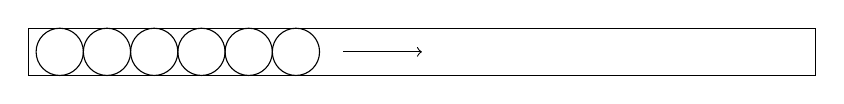
\begin{tikzpicture}
	\draw (0,0) rectangle (10,0.6);
	\draw (0.4, 0.3) circle (0.3);
	\draw (1.0, 0.3) circle (0.3);
	\draw (1.6, 0.3) circle (0.3);
	\draw (2.2, 0.3) circle (0.3);
	\draw (2.8, 0.3) circle (0.3);
	\draw (3.4, 0.3) circle (0.3);
	\draw [->](4.0, 0.3) -- (5.0, 0.3);
\end{tikzpicture}
\noindent

使用记事本打开文件,首先从磁盘读取文件数据流,
它是无编码的二进制数据(最小单元为byte)。
记事本程序根据操作系统的默认文字编码,或者智能判断出文件编码,就可以
显示文字了,

\section{BIO (Blocking IO)}
读取文件数据之后,才能处理数据。如果是单线程的代码,肯定是要等待完成数据读取
才能往下执行,不然后面的代码没有数据可以处理。所以这个过程是阻塞的,
称之为BIO(Block IO)。

JDK最早提供的文件读写方式,是基于操作系统的文件IO接口,没有提供异步的方式。
需要开发者创建一个IO线程读写和处理数据。文件类File提供了最基本的封装,
使用File可以删除、创建和遍历文件,也可以检查文件的可读写权限。

\begin{lstlisting}[language=Java]
	File file = new File("./");
	String[] list = file.list(); // 当前目录下的文件
\end{lstlisting}

\noindent
文件输入流(FileInputStream)就是从文件读取数据,
而输出流FileOutputStream就是写文件。

\subsection{字符编码}
打开记事本,写入“012345”保存。注意一下文件的编码,本书使用的是
UTF-8,然后用Hex方式查看文件内容,显示如下:
\begin{lstlisting}
	00000000:  3031 3233 3435  
\end{lstlisting}

创建并写入文件内容,可以使用FileOutputStream类提供的接口。
大家要学会查看API列表,选择一个合适的写文件函数,传入正确的参数。

\begin{lstlisting}[language=Java]
File file = new File("/Users/simbaba/Desktop/012345.txt");
       
try (FileOutputStream fos = new FileOutputStream(file)) {
		fos.write(new byte[]{0, 1, 2, 3, 4, 5});
} catch (IOException e) {
		e.printStackTrace();
}
\end{lstlisting}

\begin{table}[!htbp]\centering
	\begin{tabular}{|p{7cm}|p{5.2cm}|}
	\hline
	\multicolumn{2}{|c|}{FileOutputStream}\\
	\hline
	public void write(byte b[])&写字节数组\\
	public void write(int b) &注意:还是写1个字节\\
	public void close() &关闭文件释放文件资源\\
	public FileChannel getChannel() &获取文件通道\\
	\hline
	\end{tabular}
	\caption{FileOutputStream写文件接口}
\end{table}

\noindent
执行以上代码,再次打开文件,使用Hex的方式查看,内容如下:
\begin{lstlisting}
00000000:  0001 0203 0405          
\end{lstlisting}

\begin{table}[!htbp]\centering
	\begin{tabular}{|p{2cm}|p{2cm}|p{2cm}|}
	\hline
	十进制&十六进制&字符\\
	\hline
	48&30&0\\
	49&31&1\\
	50&32&2\\
	51&33&3\\
	\hline
	\end{tabular}
\end{table}

由以上差异,可见所谓的“012345”和实际的数据“012345”是由差别的。
UTF-8编码的“012345”,实际上对应ASCII码表中的值:
所以,读写文件的方式分为:文本、二进制方式。采用文本方式读写文件的时候,
如果遇到无法解码的数据,就会显示为乱码。通常你的笔记,都是以文本的方式
读写的,而图片和视频都是二进制的方式存储。

同样内容不同字符编码,存到文件中后的二进制数据也有可能是不一样的。
对于英文字符,使用一个字节的ASCII码就可够用了,然而其它国家
或地区的文字符号,通常超过一个字节所能表示的范围。Java的默认字符
类型char占用2个字节,使用UNICODE编码。但实际上,UNICODE仅是文字集的
编码,并不用来存储和传输用。对于英文字符,也使用2字节(16bit)表示,
将会有很多的0,譬如数字0可表示为:0x0030。

\begin{lstlisting}
	Unicode编码:0x00000030
	UTF8编码:0x30
	UTF16编码:0xFEFF0030
	UTF32编码:0x0000FEFF00000030	
\end{lstlisting}

所以,编码和字符集的对应关系如果搞错,就会出现乱码的情况。不同的字符编码
有一定的规律,譬如FEFF标志、最高为1等。
记住这些特点,可用来自动检测数据流/文件流的编码,才能正确显示文本内容。

\begin{lstlisting}[language=java]
	try (FileInputStream fis = new FileInputStream(file)) {
    int len = fis.available();
    byte[] bytes = new byte[len];
    fis.read(bytes);

    System.out.println(Hex.encodeHexString(bytes));
    String text = new String(bytes, Charset.forName("UTF-8"));
    System.out.println(text);
	} catch (IOException e) {
			e.printStackTrace();
	}
\end{lstlisting}
\noindent
以上代码输出:e88194e9809a(UTF-8字符编码)、联通(实际文字内容)。

\subsection{IO架构}
在面向对象章节,曾经介绍过IO的架构,涉及到的对象类型和继承关系。
\figref{fig:part1_io_framewk}只含有字节输入的相关类,输出和此类似。

\begin{figure}[!htb]
	\begin{center}
	\begin{tikzpicture}
	\umlsimpleclass{Inputstream}
	\umlsimpleclass[x=4, y=-1, anchor=west]{FilterInputStream}
	\umlsimpleclass[x=0.5, y=-2, anchor=west]{ByteArrayInputstream}
	\umlsimpleclass[x=0.5, y=-3, anchor=west]{StringBufferInputstream}
	\umlsimpleclass[x=0.5, y=-4, anchor=west]{FileInputStream}
	\umlsimpleclass[x=0.5, y=-5, anchor=west]{ObjectInputStream}
	\umlsimpleclass[x=0.5, y=-6, anchor=west]{SequenceInputStream}
	
	\umlsimpleclass[x=7, y=-2, anchor=west]{BufferedInputstream}
	\umlsimpleclass[x=7, y=-3, anchor=west]{DataInputstream}
	\umlsimpleclass[x=7, y=-4, anchor=west]{LineNumberInputstream}
	\umlsimpleclass[x=7, y=-5, anchor=west]{PushbackInputstream}
	
	\umlVHVinherit[arm2=-4cm]{FileInputStream}{Inputstream}
	\umlVHVinherit[arm2=-2cm]{ByteArrayInputstream}{Inputstream}
	\umlVHVinherit[arm2=-3cm]{StringBufferInputstream}{Inputstream}
	\umlVHVinherit[arm2=-1cm]{FilterInputStream}{Inputstream}
	\umlVHVinherit[arm2=-5cm]{ObjectInputStream}{Inputstream}
	\umlVHVinherit[arm2=-6cm]{SequenceInputStream}{Inputstream}
	
	\umlVHVinherit[arm2=-1cm]{BufferedInputstream}{FilterInputStream}
	\umlVHVinherit[arm2=-2cm]{DataInputstream}{FilterInputStream}
	\umlVHVinherit[arm2=-3cm]{LineNumberInputstream}{FilterInputStream}
	\umlVHVinherit[arm2=-4cm]{PushbackInputstream}{FilterInputStream}
	\end{tikzpicture}
	\end{center}
	\caption{IO继承图}
	\label{fig:part1_io_framewk}
\end{figure}

\noindent
最基本最常用的是FileInputStream,其它根据需要合理选择。
输入流(Inputstream)不仅限于文件,也可以是从数组、字符串甚至是对象。
作为(as a)一个输入流,就是要实现Inputstream的接口。
我们可以实现一个随机数输入流,每次read都返回一个随机整数,如下:
\vspace{0.3cm}
\begin{lstlisting}[language=Java]
	//仅仅是示例代码
	RandomInputstream ris = new RandomInputstream();
	ris.setRange(1, 10); // 设置范围
	int n = ris.read(); // 返回一个随机数
\end{lstlisting}
\noindent
如上代码,RandomInputstream是一个无限流,没有文件结尾。
\figref{fig:part1_io_framewk}中,每个输入流的具体用法,可参考下表:
\vspace{0.3cm}
\begin{table}[!htbp]\centering
	\lstset{frame=none, language=Java}
	\begin{tabular}{|p{4cm}|p{9cm}|}
	\hline
	IO类&示例\\ 
	\hline
	ByteArrayInputstream \newline 包装一个byte[]作为输入&
\begin{lstlisting}
	b = new byte[]{100,2,3,4};
	bInput = new ByteArrayInputStream(b);
	int n1 = bInput.read(); //100
	int n2 = bInput.read(); //2
\end{lstlisting} \\
	\hline
	StringBufferInputstream \newline 把字符串作为输入&
\begin{lstlisting}
	bInput = new StringBufferInputStream("123456");
	int n1 = bInput.read() - '0'; //1
	char n2 = (char) bInput.read(); //2
\end{lstlisting} \\
	\hline
	FileInputStream \newline 读文件& 略。\\
	\hline
	ObjectInputStream \newline 从流中获取一个对象&参考代码见后。\\
	\hline
	SequenceInputStream \newline 合并流&参考代码见后。\\
	\hline
	\end{tabular}
\end{table}

\noindent
ByteArrayOutputStream的参考代码:
\begin{lstlisting}[language=Java]
	Student student = new Student(10, "jim");

	ByteArrayOutputStream bai = new ByteArrayOutputStream(100);
	ObjectOutputStream oos = new ObjectOutputStream(bai);
	oos.writeObject(student);
	oos.close();
	byte[] dst = bai.toByteArray();

	ByteArrayInputStream bais = new ByteArrayInputStream(dst);
	ObjectInputStream bInput = new ObjectInputStream(bais);
	Student object = (Student) bInput.readObject();
	System.out.printf("name=%s, age=%d", object.name, object.age);

	// SequenceInputStream 示例
	byte[] b1 = new byte[]{1, 2, 3, 4};
	ByteArrayInputStream bis1 = new ByteArrayInputStream(b1);
	byte[] b2 = new byte[]{10, 20, 30, 40};
	ByteArrayInputStream bis2 = new ByteArrayInputStream(b2);

	SequenceInputStream sis = new SequenceInputStream(bis1, bis2);
	System.out.println("a = " + sis.available()); // 4

	int b;
	while ((b=sis.read()) != -1) {
			System.out.println(b); // 1 2 3 4 10 20 30 40
	}
\end{lstlisting}
\noindent

关于Object对象串行化,需要注意\lstinline{serialVersionUID}
和\lstinline{transient}的作用。
不同VersionUID的数据文件,是不能再读取成对象实例的。
在Student中添加一个sex字段,修饰为\lstinline{transient}就不会保存到文件中了。
如果保存的时候serialVersionUID=1,后来修改为2L就会导致加载对象失败。
\vspace{0.6cm}

\begin{lstlisting}[language=Java]
	class Student implements Serializable{
			static final long serialVersionUID = 2L;
			int age;
			String name;
			transient boolean sex;
			Student(int age, String name){
					this.age = age;
					this.name = name;
					this.sex = true;
			}
	}
	FileInputStream fis = new FileInputStream("student.txt");
	ObjectInputStream bInput = new ObjectInputStream(fis);
	Student o = (Student) bInput.readObject();
	// 打印o.sex=false而不是true
	System.out.printf("name=%s, age=%d, sex=%b", o.name, o.age, o.sex);
\end{lstlisting}

对传统的读写方式介绍就介绍这么多,只要能掌握FileInputStream的用法,
其它都与此相似,因为都是复用的InputStream的接口。
最简单的解决办法,就是单独创建一个IO线程,在这个线程里完成数据的读写和处理。

对于字符流有Reader和Writer两个基类,提供了最基本的读写接口。
谈到字符就离不开编码,不是所有的文件都能显示为可读内容。
譬如,你打开一张图片,尽管也能看到一些汉字,但都是乱七八糟的还夹杂着
很多未知符号。如下\figref{fig:part1_io_char_framewk}和字节流有很相似的
类继承结构,主要的差别是Reader/Writer依赖字节流完成读写,所以最底层还是
先读入字节然后根据字符编码解析文字。

\begin{figure}[!htb]
	\begin{center}
	\begin{tikzpicture}
	\umlsimpleclass{Reader}
	\umlsimpleclass[x=2, anchor=west]{InputPutStream}
	\umlsimpleclass[y=-1.5, anchor=north]{FileReader}
	\umlsimpleclass[x=3.5, y=-1.5, anchor=north]{CharArrayReader}
	\umlsimpleclass[x=7, y=-1.5, anchor=north]{FilterReader}

	\umlsimpleclass[y=-3]{Writer}
	\umlsimpleclass[y=-3, x=2, anchor=west]{OutPutStream}
	\umlsimpleclass[y=-5]{FileWriter}
	\umlsimpleclass[x=3.5, y=-5]{CharArrayWriter}
	\umlsimpleclass[x=7, y=-5]{FilterWriter}

	\umluniassoc{Reader}{InputPutStream}
	\umluniassoc{Writer}{OutPutStream}
	\umlVHVinherit[arm2=-2cm]{FileReader}{Reader}
	\umlVHVinherit[arm2=-1cm]{CharArrayReader}{Reader}
	\umlVHVinherit[arm2=-2cm]{FileWriter}{Writer}
	\umlVHVinherit[arm2=-1cm]{CharArrayWriter}{Writer}
	\umlVHVinherit[arm2=-1cm]{FilterReader}{Reader}
	\umlVHVinherit[arm2=-1cm]{FilterWriter}{Writer}
	\end{tikzpicture}
	\end{center}
	\caption{字符流架构}
	\label{fig:part1_io_char_framewk}
\end{figure}

\begin{lstlisting}[language=Java]
	FileWriter fw = new FileWriter("student.txt");
	fw.write("张三,10岁");
	fw.close();

	FileReader fr = new FileReader("student.txt");
	BufferedReader br = new BufferedReader(fr);
	String text = br.readLine();
	System.out.println(text);
	fr.close();
\end{lstlisting}

以上这段代码,使用的系统默认的编码。如果把上述文件另外为GBK编码,
上述代码就会显示乱码甚至异常。

\begin{lstlisting}[language=Java]
	String str = "张三,10岁";
	byte[] bytes = str.getBytes("GBK");

	System.out.println(Hex.encodeHexString(bytes));
	String text = new String(bytes, Charset.forName("UTF-8"));
	System.out.println(text);
	// 输出:
	// d5c5c8fda3ac3130cbea
	// ??????10??
\end{lstlisting}

\section{Net编程和AIO (Asynchronous IO)}
IO的阻塞读写方式,在很多场合都不适用,它会让当前线程甚至程序卡住。
\noindent
举一个简单的例子:从大于1G的文件里面查找数据,或者从网络下载一个页面。
网络程序也提供了Inputstream、OutputStream对象,
有了它们就能像文件IO一样上传和下载数据。

\begin{lstlisting}[language=Java]
	Socket socket=new Socket(InetAddress.getByName("www.baidu.com"),80);
	OutputStream os=socket.getOutputStream();
	OutputStreamWriter osw=new OutputStreamWriter(os);
	BufferedWriter bw=new BufferedWriter(osw);

	//最基本的请求头
	bw.write("GET / HTTP/1.1\r\n");
	bw.write("Host: www.baidu.com\r\n\r\n");
	bw.flush();
	socket.shutdownOutput();

	//读取response
	InputStream is=socket.getInputStream();
	BufferedReader br=new BufferedReader(new InputStreamReader(is));
	String str=null;
	while((str=br.readLine())!=null){
			System.out.println(str);
	}
	socket.close();
\end{lstlisting}

上述下载Web页面的代码,用到了HTTP GET指令。实际下载代码,可以直接使用
HttpClient或者URL类型提供的接口。

\begin{lstlisting}[language=Java]
	// 注意带上http以便URL识别协议
	URL url=new URL("http://www.baidu.com");
	InputStream is= url.openStream();;

	//读取response
	BufferedReader br=new BufferedReader(new InputStreamReader(is));
	String str=null;
	while((str=br.readLine())!=null){
			System.out.println(str);
	}
	is.close();
  //---------------------------------------
	HttpGet http=new HttpGet("https://www.baidu.com");
	try (
			CloseableHttpClient httpClient = HttpClients.createDefault();
			CloseableHttpResponse response = httpClient.execute(http);
	) {
			HttpEntity entity = response.getEntity();
			String page = EntityUtils.toString(entity, "UTF-8");
			System.out.println(page);
	} catch (IOException e) {
			e.printStackTrace();
	}
\end{lstlisting}

\noindent
网络不畅会导致上传、下载阻塞,所以不适合在主线程做。
对于UI交互类应用,主线程要能响应用户操作,即使在等待Web网页下载也不能
卡住用户的的各种点击,尤其是“取消”。

\section{NIO (New/Non-Blocking IO)}
NIO(New Input/ Output)是在JDK1.4引入的基于通道和缓冲区的I/O方式,
它是一种非阻塞的IO模型,使用Selector轮询IO事件,但不阻塞当前线程往下执行。
Selector作为选择器,也称为多路复用器,是NIO的核心组件,
用于检查一个或多个NIO Channel(通道)是否处于可读、可写,
由此实现了单个线程管理多个Channels,同时管理多个网络链接。
另外,NIO可使用Native函数直接分配堆外内存,
避免在Java堆和Native堆中来回复制数据。
\vspace{0.2cm}

\begin{tikzpicture}[level distance=2.5cm]
	\tikzstyle{level 1}=[sibling distance=2.4cm]
	\node (selector){Selector}
    child {node[rectangle,draw] {channel a}}
		child {node[rectangle,draw] {channel b}}
		child {node{...}}
		child {node[rectangle,draw] {channel d}}
		child {node[rectangle,draw] {channel e}};
	\node[below of=selector]{- 轮询 -};
\end{tikzpicture}

\noindent
如上图,Selector往往是一个无限循环,检查每个channel的状态。
这些状态包括:

\begin{table}[!htbp]\centering
	\begin{tabular}{|p{3cm}|p{6cm}|}
	\hline
	状态&说明\\
	\hline
	OP\_READ&通道中已经有了可读的数据\\
	OP\_WRITE&已经可以向通道写数据了\\
	OP\_ACCEPT&监听到了连接,可以接收这个连接了\\
	OP\_CONNECT&连接已经建立成功\\
	\hline
	\multicolumn{2}{|c|}{注意:注册了写事件,不在合适的时间去除掉,会一直触发写事件}\\
	\hline
	\end{tabular}
\end{table}

\subsection{FileChannel}
FileChannel是面向文件的通道,但无法设置为非阻塞模式,只能是阻塞模式。
值得注意的是FileChannel只是一个抽象类,提供了读、写、映射和锁住一个文件的抽象方法。
不过FileChannel是线程安全的,可以被多个并发线程使用。

FileChannel对象可通过open()方法被创建,也可通过FileInputStream、
FileOutputStream、RandomAccessFile对象的getChannel()得到。

\begin{lstlisting}[language=Java]
	Path path = Paths.get("/Users/simbaba",
                "Desktop",
					"test.txt");
	//Files.deleteIfExists(path);
	//Files.createFile(path);
	FileChannel fc =  FileChannel.open(path, StandardOpenOption.CREATE, StandardOpenOption.WRITE);

	ByteBuffer bb = ByteBuffer.allocate(10);
	bb.put(new byte[]{'1','2','3',4,5,6,7,8,9,10});
	bb.flip(); /// 非常关键,不然什么都没写!!!
	fc.write(bb);
	fc.close();
\end{lstlisting}

\section{异步Channel}
NIO提供的Selector作为“多路复用器”,用来检查一个或多个NIO Channel(通道)的状态
是否处于可读、可写。
以此实现单线程管理多个Channels,譬如可以管理多个网络链接。
通过调用Selector.open()方法创建一个Selector对象,
其它\emph{非阻塞}\footnote{FileChannel不适用Selector,
因为它没有继承SelectableChannel。}
的Channel主动注册到该Selector对象上。
通过Channel的configureBlocking()方法,使通道处于阻塞模式或非阻塞模式。